\documentclass[a4paper]{article}
\usepackage[a4paper, left=5mm, right=5mm, top=5mm, bottom=5mm]{geometry}
\usepackage[utf8]{inputenc}
\usepackage[russian]{babel}
\usepackage{graphicx}
\usepackage{indentfirst}
\usepackage{amsmath}
\usepackage{enumerate}
\usepackage{amsfonts}
\usepackage{amssymb}
\title{Задание от 2013.03.22}
\author{С.~Е.~Володин, 272 гр.}
\date{}
\begin{document}
\maketitle
\begin{enumerate}[(a)]
\item Пусть исходные строки~--- $A$, $B$: $|A|=|B|=M\equiv 2^n$. Алфавит $\Sigma=\{A,C,T,G\}$. Составим строки$A_\sigma, B_\sigma$, такие что $$A^{i}_\sigma=\left\{\begin{array}{lcr}1, & A^i=\sigma\\ 0, & else\\ \end{array}. \right.$$ Дополним $A_\sigma,B_\sigma$ нулями до строк длины $2M$:\newline
$A'_\sigma=\{A_\sigma 0\}\equiv\{A^{0}_\sigma,\dots,A^{M-1}_\sigma,0,\dots,0\}$,\newline$B'_\sigma=\{B^{inv}_\sigma 0\}\equiv\{B^{M-1}_\sigma,\dots,B^{0}_\sigma,0,\dots,0\}$.\newline
Строки $A_\sigma',B_\sigma'$ рассматриваем как коэффициенты многочленов.\newline
Посчитаем значения в точках 8-ю FFT: для $A'_A,A'_C,A'_T,A'_G,B'_A,B'_C,B'_T,B'_G$.
Перемножим значения попарно: $A'_A*B'_A,A'_C*B'_C,A'_T*B'_T,A'_G*B'_G$ и выполним 4 FFT$^{-1}$, таким образом получим коэффициенты соответствующих многочленов, которые являются количествами совпадающих символов $\sigma$ в исходных строках при фиксированном совмещении:\newline
$$c^k_\sigma=\sum\limits_{l=0}^{k} A'^l_\sigma B'^{k-l}_\sigma$$
Графически это можно представить так (изображено одно и то же умножение, просто строка B развернута во втором случае):
\begin{figure}[hr]
%	\caption{Умножение $A'_\sigma*B'_\sigma$}
	\includegraphics[width=5cm]{1.jpg}
	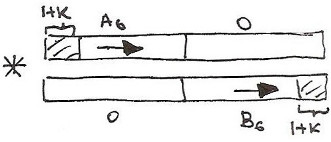
\includegraphics[width=5cm]{2.jpg}
%	\label{fig:fig1}
\end{figure}\newline
Поскольку строки циклические, нужно посчитать количество совпадающих символов и для вторых частей строк. Для этого сложим <<противоположные>> значения $c_\sigma$ (показано на рисунке ниже):
\begin{figure}[hr]
%	\caption{Умножение $A'_\sigma*B'_\sigma$}
	\includegraphics[width=5cm]{3.jpg}
%	\label{fig:fig1}
\end{figure}\newline
Таким образом, для каждой буквы $\sigma\in\Sigma$ найден массив количеств совпавших символов при каждом возможном совмещении. Сложим эти массивы для всех букв и найдем максимум в сумме за $O(M)$\newline
Получаем алгоритм, использующий 12 FFT $\blacksquare$
\item Заметим, что мы искали максимум в массиве коэффициентов $A'_A*B'_A+A'_C*B'_C+A'_T*B'_T+A'_G*B'_G$. Поэтому вместо обратного преобразования в коэффициенты соответствующих значений сложим их, то есть, весь алгоритм:\newline
Посчитаем значения в точках 8-ю FFT: для $A'_A,A'_C,A'_T,A'_G,B'_A,B'_C,B'_T,B'_G$.\newline
Получим значения многочлена $A'_A*B'_A+A'_C*B'_C+A'_T*B'_T+A'_G*B'_G$.\newline
Выполним для него FFT$^{-1}$ и сложим <<противоположные>> коэффициенты как в п. (а). Далее найдем максимум в линейном массиве (корректно, так как этот массив тот же, что и в предыдущем пункте).\newline
Всего 8 FFT на преобразование в значения и одно в коэффициенты $\Rightarrow$ 9 FFT $\blacksquare$
\end{enumerate}

\end{document}

